\documentclass[]{article}
\usepackage{lmodern}
\usepackage{amssymb,amsmath}
\usepackage{ifxetex,ifluatex}
\usepackage{fixltx2e} % provides \textsubscript
\ifnum 0\ifxetex 1\fi\ifluatex 1\fi=0 % if pdftex
  \usepackage[T1]{fontenc}
  \usepackage[utf8]{inputenc}
\else % if luatex or xelatex
  \ifxetex
    \usepackage{mathspec}
  \else
    \usepackage{fontspec}
  \fi
  \defaultfontfeatures{Ligatures=TeX,Scale=MatchLowercase}
\fi
% use upquote if available, for straight quotes in verbatim environments
\IfFileExists{upquote.sty}{\usepackage{upquote}}{}
% use microtype if available
\IfFileExists{microtype.sty}{%
\usepackage{microtype}
\UseMicrotypeSet[protrusion]{basicmath} % disable protrusion for tt fonts
}{}
\usepackage[margin=1in]{geometry}
\usepackage{hyperref}
\hypersetup{unicode=true,
            pdftitle={NOAA Storm Database - worst cases},
            pdfauthor={erickfis},
            pdfborder={0 0 0},
            breaklinks=true}
\urlstyle{same}  % don't use monospace font for urls
\usepackage{longtable,booktabs}
\usepackage{graphicx,grffile}
\makeatletter
\def\maxwidth{\ifdim\Gin@nat@width>\linewidth\linewidth\else\Gin@nat@width\fi}
\def\maxheight{\ifdim\Gin@nat@height>\textheight\textheight\else\Gin@nat@height\fi}
\makeatother
% Scale images if necessary, so that they will not overflow the page
% margins by default, and it is still possible to overwrite the defaults
% using explicit options in \includegraphics[width, height, ...]{}
\setkeys{Gin}{width=\maxwidth,height=\maxheight,keepaspectratio}
\IfFileExists{parskip.sty}{%
\usepackage{parskip}
}{% else
\setlength{\parindent}{0pt}
\setlength{\parskip}{6pt plus 2pt minus 1pt}
}
\setlength{\emergencystretch}{3em}  % prevent overfull lines
\providecommand{\tightlist}{%
  \setlength{\itemsep}{0pt}\setlength{\parskip}{0pt}}
\setcounter{secnumdepth}{5}
% Redefines (sub)paragraphs to behave more like sections
\ifx\paragraph\undefined\else
\let\oldparagraph\paragraph
\renewcommand{\paragraph}[1]{\oldparagraph{#1}\mbox{}}
\fi
\ifx\subparagraph\undefined\else
\let\oldsubparagraph\subparagraph
\renewcommand{\subparagraph}[1]{\oldsubparagraph{#1}\mbox{}}
\fi

%%% Use protect on footnotes to avoid problems with footnotes in titles
\let\rmarkdownfootnote\footnote%
\def\footnote{\protect\rmarkdownfootnote}

%%% Change title format to be more compact
\usepackage{titling}

% Create subtitle command for use in maketitle
\newcommand{\subtitle}[1]{
  \posttitle{
    \begin{center}\large#1\end{center}
    }
}

\setlength{\droptitle}{-2em}
  \title{NOAA Storm Database - worst cases}
  \pretitle{\vspace{\droptitle}\centering\huge}
  \posttitle{\par}
  \author{erickfis}
  \preauthor{\centering\large\emph}
  \postauthor{\par}
  \predate{\centering\large\emph}
  \postdate{\par}
  \date{2017 maio, 10}


\begin{document}
\maketitle

{
\setcounter{tocdepth}{3}
\tableofcontents
}
\section{Introduction}\label{introduction}

In this study we have analysed the NOAA Storm Database in order to
determine what are the worst natural catastrophic events, both in terms
of public health and in economic impact.

The U.S. National Oceanic and Atmospheric Administration's (NOAA) storm
database tracks characteristics of major storms and weather events in
the United States, including when and where they occur, as well as
estimates of any fatalities, injuries, and property damage.

The database currently contains data from January 1950 to January 2017,
as entered by NOAA's National Weather Service (NWS).

The database can be found on:

\url{https://www.ncdc.noaa.gov/stormevents/ftp.jsp}

RPubs version, with fewer plots, for Coursera:
\url{http://rpubs.com/erickfis/noaa}

\section{Objective}\label{objective}

The goal of this study is to answer the questions:

\begin{enumerate}
\def\labelenumi{\arabic{enumi}.}
\item
  Across the United States, which types of events were the most harmful
  with respect to population health ever recorded in a single
  occurrence?
\item
  Which types of events caused most harm to population health along all
  those years?
\item
  Which types of events had the greatest economic consequences in a
  single occurrence?
\item
  Which types of events had the greatest economic consequences along all
  those years?
\item
  Which were the places that were subject to the greatest losses, both
  in terms of human health and economic losses.
\end{enumerate}

\section{Methods}\label{methods}

To answer each one of those questions, we did a very simple
\textbf{descriptive analysis} of data.

We used R tools to filter, sort and combine data, so we could get the
total sum of fatalities, injuries and economic losses.

\section{Data Processing}\label{data-processing}

In order to answer our questions, the original database needed to be
treated from its raw form to a more useful format.

\subsubsection{New files to download and process data
again:}\label{new-files-to-download-and-process-data-again}

\begin{verbatim}
    StormEvents_details-ftp_v1.0_d2006_c20170405.csv.gz, StormEvents_details-ftp_v1.0_d2015_c20170216.csv.gz, StormEvents_details-ftp_v1.0_d1951_c20160223.csv.gz, StormEvents_details-ftp_v1.0_d1952_c20160223.csv.gz, StormEvents_details-ftp_v1.0_d1955_c20160223.csv.gz, StormEvents_details-ftp_v1.0_d1960_c20160223.csv.gz, StormEvents_details-ftp_v1.0_d1961_c20160223.csv.gz, StormEvents_details-ftp_v1.0_d1962_c20160223.csv.gz, StormEvents_details-ftp_v1.0_d1963_c20160223.csv.gz, StormEvents_details-ftp_v1.0_d1964_c20160223.csv.gz, StormEvents_details-ftp_v1.0_d1970_c20160223.csv.gz, StormEvents_details-ftp_v1.0_d1975_c20160223.csv.gz, StormEvents_details-ftp_v1.0_d1979_c20160223.csv.gz, StormEvents_details-ftp_v1.0_d1981_c20160223.csv.gz, StormEvents_details-ftp_v1.0_d1982_c20160223.csv.gz, StormEvents_details-ftp_v1.0_d1984_c20160223.csv.gz, StormEvents_details-ftp_v1.0_d1991_c20160223.csv.gz, StormEvents_details-ftp_v1.0_d1992_c20160223.csv.gz, StormEvents_details-ftp_v1.0_d1993_c20160223.csv.gz, StormEvents_details-ftp_v1.0_d1994_c20160223.csv.gz, StormEvents_details-ftp_v1.0_d1997_c20160223.csv.gz, StormEvents_details-ftp_v1.0_d1999_c20160223.csv.gz, StormEvents_details-ftp_v1.0_d2000_c20160223.csv.gz, StormEvents_details-ftp_v1.0_d2002_c20160223.csv.gz, StormEvents_details-ftp_v1.0_d2004_c20160223.csv.gz, StormEvents_details-ftp_v1.0_d2007_c20160223.csv.gz, StormEvents_details-ftp_v1.0_d2009_c20160223.csv.gz, StormEvents_details-ftp_v1.0_d2010_c20160223.csv.gz, StormEvents_details-ftp_v1.0_d2011_c20160223.csv.gz, StormEvents_details-ftp_v1.0_d2013_c20170419.csv.gz, StormEvents_details-ftp_v1.0_d2017_c20170419.csv.gz, StormEvents_details-ftp_v1.0_d1953_c20160223.csv.gz, StormEvents_details-ftp_v1.0_d1954_c20160223.csv.gz, StormEvents_details-ftp_v1.0_d1956_c20160223.csv.gz, StormEvents_details-ftp_v1.0_d1957_c20160223.csv.gz, StormEvents_details-ftp_v1.0_d1958_c20160223.csv.gz, StormEvents_details-ftp_v1.0_d1959_c20160223.csv.gz, StormEvents_details-ftp_v1.0_d1965_c20160223.csv.gz, StormEvents_details-ftp_v1.0_d1966_c20160223.csv.gz, StormEvents_details-ftp_v1.0_d1967_c20160223.csv.gz, StormEvents_details-ftp_v1.0_d1968_c20160223.csv.gz, StormEvents_details-ftp_v1.0_d1969_c20160223.csv.gz, StormEvents_details-ftp_v1.0_d1971_c20160223.csv.gz, StormEvents_details-ftp_v1.0_d1972_c20160223.csv.gz, StormEvents_details-ftp_v1.0_d1973_c20160223.csv.gz, StormEvents_details-ftp_v1.0_d1974_c20160223.csv.gz, StormEvents_details-ftp_v1.0_d1976_c20160223.csv.gz, StormEvents_details-ftp_v1.0_d1977_c20160223.csv.gz, StormEvents_details-ftp_v1.0_d1978_c20160223.csv.gz, StormEvents_details-ftp_v1.0_d1980_c20160223.csv.gz, StormEvents_details-ftp_v1.0_d1983_c20160223.csv.gz, StormEvents_details-ftp_v1.0_d1985_c20160223.csv.gz, StormEvents_details-ftp_v1.0_d1986_c20160223.csv.gz, StormEvents_details-ftp_v1.0_d1987_c20160223.csv.gz, StormEvents_details-ftp_v1.0_d1988_c20160223.csv.gz, StormEvents_details-ftp_v1.0_d1989_c20160223.csv.gz, StormEvents_details-ftp_v1.0_d1990_c20160223.csv.gz, StormEvents_details-ftp_v1.0_d1995_c20160223.csv.gz, StormEvents_details-ftp_v1.0_d1996_c20160223.csv.gz, StormEvents_details-ftp_v1.0_d1998_c20160223.csv.gz, StormEvents_details-ftp_v1.0_d2003_c20160223.csv.gz, StormEvents_details-ftp_v1.0_d2008_c20160223.csv.gz, StormEvents_details-ftp_v1.0_d2012_c20160223.csv.gz, StormEvents_details-ftp_v1.0_d2016_c20170419.csv.gz, StormEvents_details-ftp_v1.0_d2005_c20170405.csv.gz, StormEvents_details-ftp_v1.0_d2014_c20161118.csv.gz, StormEvents_details-ftp_v1.0_d1950_c20170120.csv.gz
\end{verbatim}

The necessary transformations were:

\begin{itemize}
\tightlist
\item
  sanitized var names
\item
  evaluated duration of events
\item
  evaluated damages values according to multipliers provided
\item
  sanitized and grouped similar events: strong snow, heavy snow and
  light snow all became just ``snow''
\item
  sanitized county names
\end{itemize}

This database has 1419673 observations. Each observation corresponds to
an event occurrence.

To determine the most harmful events to human health, we checked the
variables related to human health, which are ``fatalities'' and
``injuries''.

To determine the most harmful events to economy, we checked the
variables related to economic measures, from ``propdmg'' through
``cropdmgexp''.

Also, in order to analyse various occurrences of the same event, we
measured the duration of the event, its magnitude and where the event
occurred (state and county name).

This is a really big database whose data has been being registered by a
lot of different people since 1950. Thus, as expected, there are
variations on how people registered events.

For example, the string ``snow'' was used to register a lot of events.
They are the same type of event, but count as different:

This is why we decided to filter those events: we grouped them by its
common strings.

\section{Human health: the most harmfull
events}\label{human-health-the-most-harmfull-events}

We have determined what events did more harm to human health.

There were occurrences that caused zero fatalities but a lot of
injuries. The inverse is also true, so we did a separate analysis to
fatal and non-fatal events.

\subsection{Fatal Occurrences}\label{fatal-occurrences}

\subsubsection{Most fatal in a single
occurrence}\label{most-fatal-in-a-single-occurrence}

Most fatal in a single occurrence

In order to determine what were the most fatal events in a single
occurrence, we need to see how fatalities are distributed along the
occurrences.

Looking at this distribution, we can infer that the vast majority of
those occurrences were not fatal at all: \textbf{99.2\% occurrences
didn't caused any fatalities.}

On the other hand, fatal occurrences had to have at least 1 fatality.

Now, among the fatal occurrences, we are interested in the ones whose
fatalities are beyond the confidence interval, ie. above 99\% of the
most common values.

Looking at this distribution, we can infer that \textbf{99.8\% of the
fatal occurrences caused up to 57.04 fattalities}.

Distribution plots

\begin{figure}[htbp]
\centering
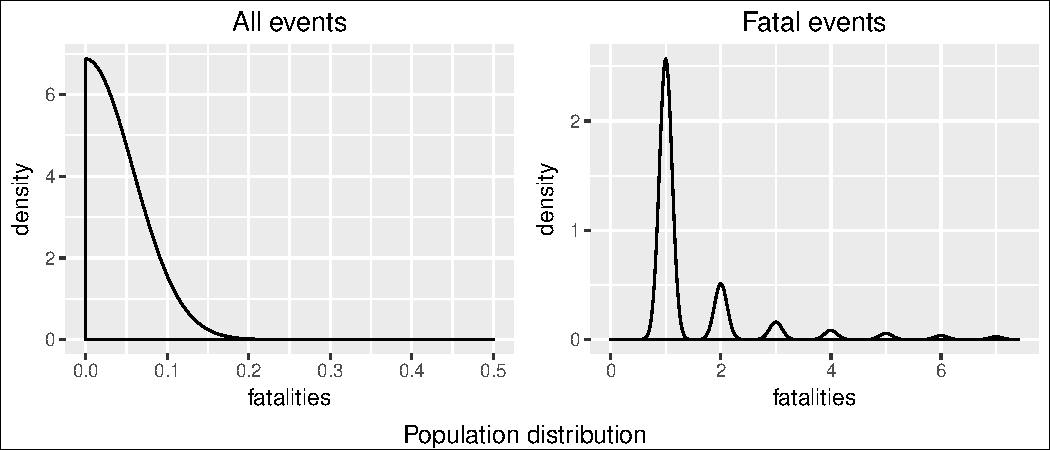
\includegraphics{readme_files/figure-latex/fatal-distr-4-1.pdf}
\caption{Population distribution for fatalities / occurrences}
\end{figure}

In this study, we looked on the 1\% deadliest occurrences.

\begin{longtable}[]{@{}rlllrllrrr@{}}
\caption{Worst fatal occurrences}\tabularnewline
\toprule
rank & event & magnitude & day & duration & state & countyname &
fatalities & mean & median\tabularnewline
\midrule
\endfirsthead
\toprule
rank & event & magnitude & day & duration & state & countyname &
fatalities & mean & median\tabularnewline
\midrule
\endhead
1 & HURRICANE & & 2005-08-28 & 0S & LOUISIANA & ORLEANS & 638 & 1.904628
& 1\tabularnewline
2 & TORNADO & & 2011-05-22 & 0S & MISSOURI & JASPER & 161 & 1.904628 &
1\tabularnewline
3 & HURRICANE & & 2005-08-28 & 0S & LOUISIANA & LOWER.ST..BERNARD & 140
& 1.904628 & 1\tabularnewline
4 & TORNADO & 0 & 1953-06-08 & 0S & MICHIGAN & GENESEE & 116 & 1.904628
& 1\tabularnewline
5 & TORNADO & 0 & 1953-05-11 & 0S & TEXAS & MCLENNAN & 114 & 1.904628 &
1\tabularnewline
6 & HURRICANE & & 2005-08-28 & 0S & MISSISSIPPI & HARRISON & 97 &
1.904628 & 1\tabularnewline
7 & HEAT & & 1999-07-28 & 0S & ILLINOIS & COOK & 93 & 1.904628 &
1\tabularnewline
8 & TORNADO & 0 & 1953-06-09 & 0S & MASSACHUSETTS & WORCESTER & 90 &
1.904628 & 1\tabularnewline
9 & TORNADO & 0 & 1955-05-25 & 0S & KANSAS & COWLEY & 75 & 1.904628 &
1\tabularnewline
10 & HEAT & & 1999-07-04 & 0S & PENNSYLVANIA & PHILADELPHIA & 58 &
1.904628 & 1\tabularnewline
\bottomrule
\end{longtable}

\begin{figure}[htbp]
\centering
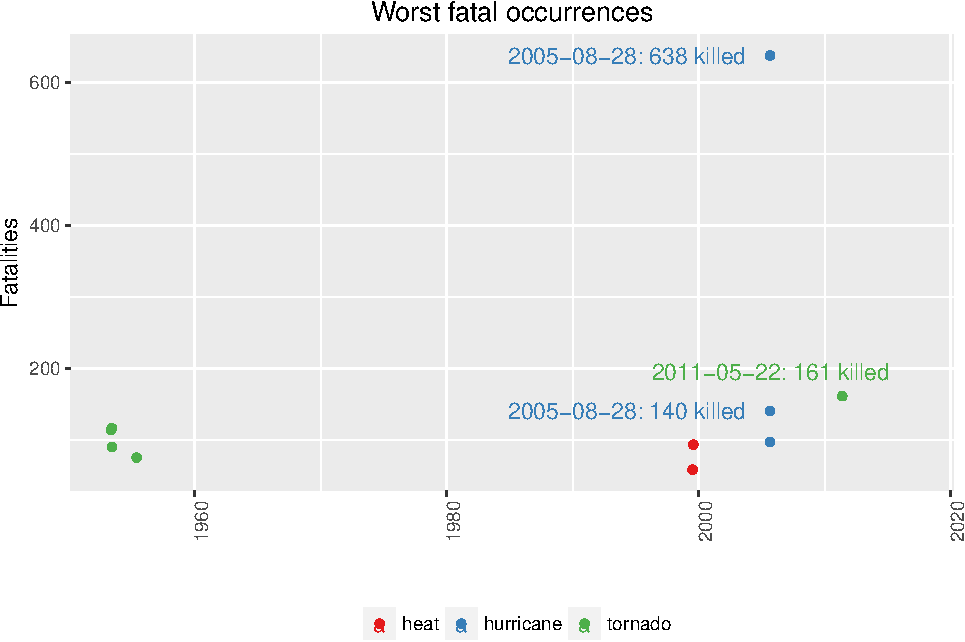
\includegraphics{readme_files/figure-latex/fatal-plot-single-1.pdf}
\caption{Worst fatal occurrences}
\end{figure}

The single most fatal event was a \textbf{HURRICANE, that occurred in
LOUISIANA, ORLEANS, on 2005-08-28, killing 638 people.}

However, if we compare this single awful event to the mean of fatalities
caused, we see that this is very unlikely to happen.

\subsubsection{Most fatal in all time}\label{most-fatal-in-all-time}

Most fatal in all time

Notice that are several occurrences of the same type of event along the
time.

Therefore, in order to know which is the worst type of event along all
the years, we summed up the fatalities caused by each one of occurrences
of this events.

Notice that we are interested only in the worst of them, ie, the ones
which are above the mean.

\begin{longtable}[]{@{}rlrrr@{}}
\caption{Total fatalities by event}\tabularnewline
\toprule
rank & event & total & mean & median\tabularnewline
\midrule
\endfirsthead
\toprule
rank & event & total & mean & median\tabularnewline
\midrule
\endhead
1 & TORNADO & 5873 & 677.5714 & 184\tabularnewline
2 & HEAT & 2854 & 677.5714 & 184\tabularnewline
3 & WIND & 2304 & 677.5714 & 184\tabularnewline
4 & FLOOD & 1944 & 677.5714 & 184\tabularnewline
5 & WINTER & 1196 & 677.5714 & 184\tabularnewline
6 & HURRICANE & 1128 & 677.5714 & 184\tabularnewline
7 & LIGHTNING & 833 & 677.5714 & 184\tabularnewline
8 & RIP CURRENT & 798 & 677.5714 & 184\tabularnewline
\bottomrule
\end{longtable}

\begin{figure}[htbp]
\centering
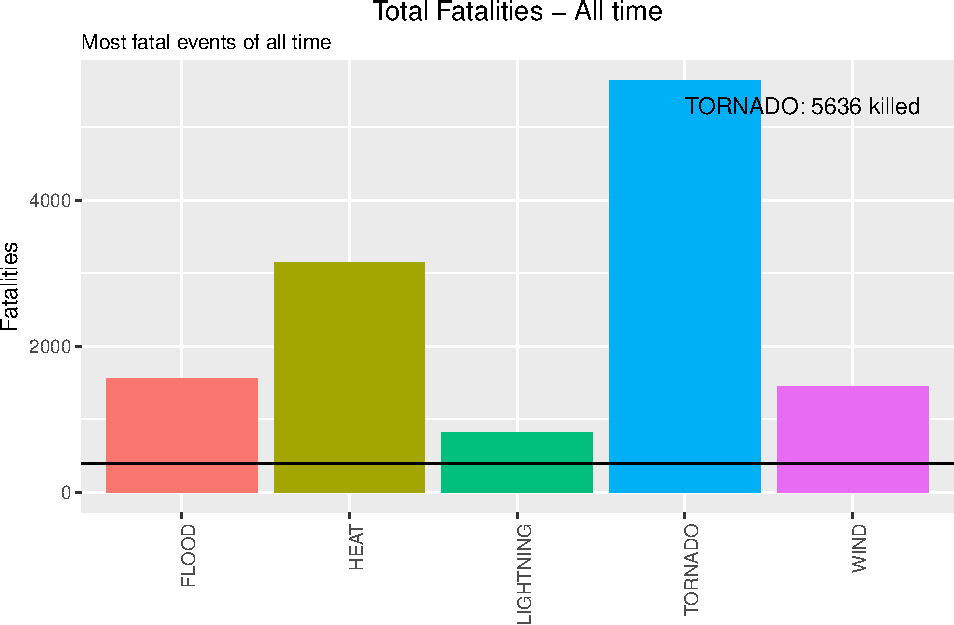
\includegraphics{readme_files/figure-latex/fatal-plot-alltime-1.pdf}
\caption{Total fatalities by event}
\end{figure}

The most fatal event along the time is the \textbf{TORNADO. It has
killed 5873 people until now.}

\subsubsection{Least fatal events}\label{least-fatal-events}

Just for curiosity, these are the less fatal among the fatal events:

\begin{longtable}[]{@{}rlr@{}}
\caption{Least fatal events}\tabularnewline
\toprule
rank & event & total\tabularnewline
\midrule
\endfirsthead
\toprule
rank & event & total\tabularnewline
\midrule
\endhead
28 & TROPICAL DEPRESSION & 1\tabularnewline
27 & DENSE SMOKE & 2\tabularnewline
26 & SLEET & 2\tabularnewline
25 & WATERSPOUT & 2\tabularnewline
24 & COLD & 4\tabularnewline
23 & DUST DEVIL & 4\tabularnewline
22 & SLIDE & 4\tabularnewline
21 & SNEAKERWAVE & 14\tabularnewline
20 & HAIL & 20\tabularnewline
19 & TIDE & 22\tabularnewline
\bottomrule
\end{longtable}

\subsection{Injuring Occurrences}\label{injuring-occurrences}

\subsubsection{Most injuring in a single
occurrence}\label{most-injuring-in-a-single-occurrence}

Most injuring in a single occurrence

In order to determine what were the most injuring events in a single
occurrence, we need to see how injuries are distributed along the
occurrences.

Looking at this distribution, we can infer that the vast majority of
those occurrences were not injuring at all: \textbf{98.5\% occurrences
didn't caused any injuries}

On the other hand, injuring occurrences had to have at least 1 injury.

Now, among the injuring occurrences, we are interested in the ones whose
harm is beyond the confidence interval, ie. above 99\% of the most
common values.

Looking at this distribution, we can infer that \textbf{99.8\% of the
injuring occurrences caused up to 500 injuries}.

Distribution plots

\begin{figure}[htbp]
\centering
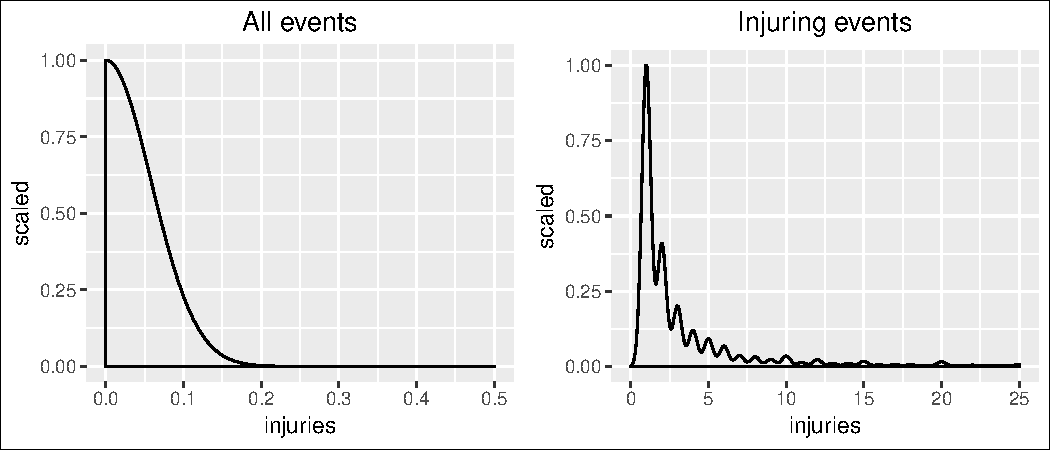
\includegraphics{readme_files/figure-latex/inj-distribution-1.pdf}
\caption{Population distribution for Injuries / occurrences}
\end{figure}

In this study, we looked on the 1\% most injuring occurrences.

\begin{longtable}[]{@{}rlllrllrrr@{}}
\caption{Worst injuring occurrences}\tabularnewline
\toprule
rank & event & magnitude & day & duration & state & countyname &
injuries & mean & median\tabularnewline
\midrule
\endfirsthead
\toprule
rank & event & magnitude & day & duration & state & countyname &
injuries & mean & median\tabularnewline
\midrule
\endhead
1 & HURRICANE & & 2008-09-12 & 0S & TEXAS & HARRIS & 2400 & 7.570462 &
2\tabularnewline
2 & TORNADO & 0 & 1979-04-10 & 0S & TEXAS & WICHITA & 1700 & 7.570462 &
2\tabularnewline
3 & TORNADO & 0 & 1953-06-09 & 0S & MASSACHUSETTS & WORCESTER & 1228 &
7.570462 & 2\tabularnewline
4 & TORNADO & 0 & 1974-04-03 & 0S & OHIO & GREENE & 1150 & 7.570462 &
2\tabularnewline
5 & TORNADO & & 2011-05-22 & 0S & MISSOURI & JASPER & 1150 & 7.570462 &
2\tabularnewline
6 & FLOOD & & 1998-10-17 & 0S & TEXAS & COMAL & 800 & 7.570462 &
2\tabularnewline
7 & TORNADO & & 2011-04-27 & 0S & ALABAMA & TUSCALOOSA & 800 & 7.570462
& 2\tabularnewline
8 & TORNADO & 0 & 1953-06-08 & 0S & MICHIGAN & GENESEE & 785 & 7.570462
& 2\tabularnewline
9 & HURRICANE & & 2004-08-13 & 0S & FLORIDA & CHARLOTTE & 700 & 7.570462
& 2\tabularnewline
10 & TORNADO & & 2011-04-27 & 0S & ALABAMA & JEFFERSON & 700 & 7.570462
& 2\tabularnewline
11 & FLOOD & & 1998-10-17 & 0S & TEXAS & BEXAR & 600 & 7.570462 &
2\tabularnewline
12 & TORNADO & 0 & 1953-05-11 & 0S & TEXAS & MCLENNAN & 597 & 7.570462 &
2\tabularnewline
13 & TORNADO & 0 & 1965-04-11 & 0S & INDIANA & HOWARD & 560 & 7.570462 &
2\tabularnewline
14 & HEAT & & 2007-08-04 & 0S & MISSOURI & ST..LOUIS & 519 & 7.570462 &
2\tabularnewline
15 & TORNADO & 0 & 1966-03-03 & 0S & MISSISSIPPI & HINDS & 504 &
7.570462 & 2\tabularnewline
\bottomrule
\end{longtable}

\begin{figure}[htbp]
\centering
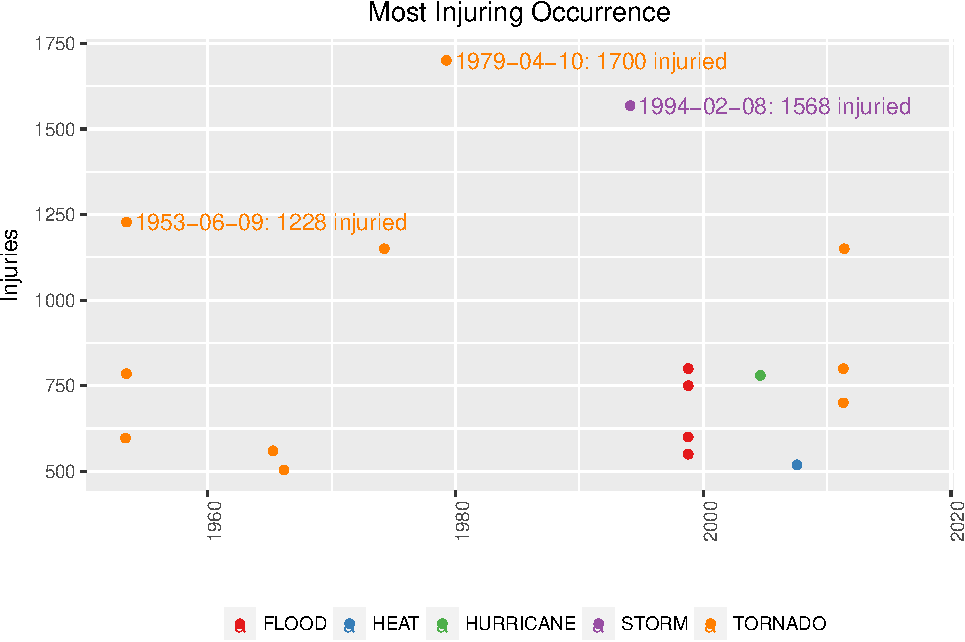
\includegraphics{readme_files/figure-latex/injuring-single-plot-1.pdf}
\caption{Worst injuring occurrences}
\end{figure}

The single most injuring event was a \textbf{HURRICANE, that occurred in
TEXAS, HARRIS, on 2008-09-12, injuring 2400 people.}

However, if we compare this single awful event to the mean of injuries
caused, we see that this is very unlikely to happen.

\subsubsection{Most injuring in all
time}\label{most-injuring-in-all-time}

Most injuring in all time

Notice that are several occurrences of the same type of event along the
time.

Therefore, in order to know which is the worst type of event along all
the years, we summed up the injuries caused by each one of occurrences
of this events.

Notice that we are interested only in the worst of them, ie, the ones
which are above the mean.

\begin{longtable}[]{@{}rlrrr@{}}
\caption{Total injuries by event}\tabularnewline
\toprule
rank & event & total & mean & median\tabularnewline
\midrule
\endfirsthead
\toprule
rank & event & total & mean & median\tabularnewline
\midrule
\endhead
1 & TORNADO & 94614 & 5200.419 & 316\tabularnewline
2 & HEAT & 15436 & 5200.419 & 316\tabularnewline
3 & WIND & 13439 & 5200.419 & 316\tabularnewline
4 & FLOOD & 8806 & 5200.419 & 316\tabularnewline
5 & WINTER & 8224 & 5200.419 & 316\tabularnewline
\bottomrule
\end{longtable}

The most injuring event along the time is the \textbf{TORNADO. It has
injuried 94614 people until now.}

\begin{figure}[htbp]
\centering
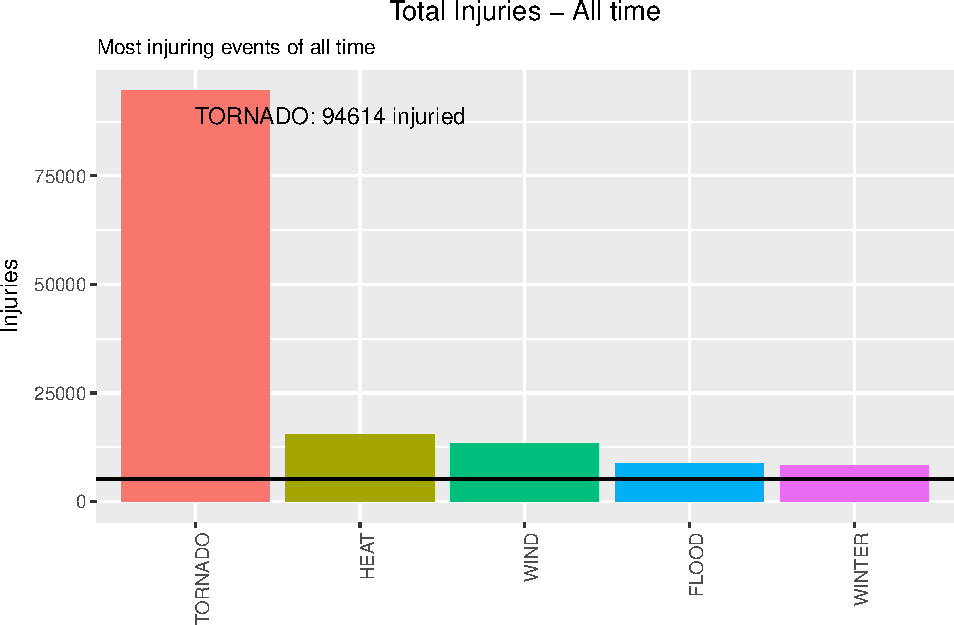
\includegraphics{readme_files/figure-latex/injuring-all-plot-1.pdf}
\caption{Total Injuries by event}
\end{figure}

\subsubsection{Least injuring events}\label{least-injuring-events}

Just for curiosity, lets show now what are the less injuring among the
injuring events:

\begin{longtable}[]{@{}rlr@{}}
\caption{Least injuring events}\tabularnewline
\toprule
rank & event & total\tabularnewline
\midrule
\endfirsthead
\toprule
rank & event & total\tabularnewline
\midrule
\endhead
31 & FUNNEL & 3\tabularnewline
30 & TROPICAL DEPRESSION & 3\tabularnewline
29 & WATERSPOUT & 3\tabularnewline
28 & OTHER & 4\tabularnewline
27 & DROUGHT & 8\tabularnewline
26 & SLEET & 10\tabularnewline
25 & SNEAKERWAVE & 11\tabularnewline
24 & SLIDE & 13\tabularnewline
23 & COLD & 15\tabularnewline
22 & DENSE SMOKE & 17\tabularnewline
\bottomrule
\end{longtable}

\section{Economy: the the most harmfull
events}\label{economy-the-the-most-harmfull-events}

We have determined what events did more harm to economy, both in terms
of property and crops damage.

There were events that causes zero property damage but a lot of crop
damage. The inverse is also true, so we did a separate analysis to
property VS crop damaging events.

\subsection{Property losses}\label{property-losses}

\subsubsection{Most Property Damaging event in a single
occurrence}\label{most-property-damaging-event-in-a-single-occurrence}

In order to determine what were the most property damaging events in a
single occurrence, we need to see how damages are distributed along the
occurrences.

Looking at this distribution, we can infer that 99.8\% of the
occurrences caused less than \textbf{\$40,000,000 in losses}.

On the other hand, damaging occurrences had to have damages above zero.

Now, among the damaging occurrences, we are interested in the ones whose
damages are above 99.8\% of the most common values.

Looking at this distribution, we can infer that \textbf{99.8\% of the
damaging occurrences caused up to \$128,960,700 in losses}.

Distribution plots

\begin{figure}[htbp]
\centering
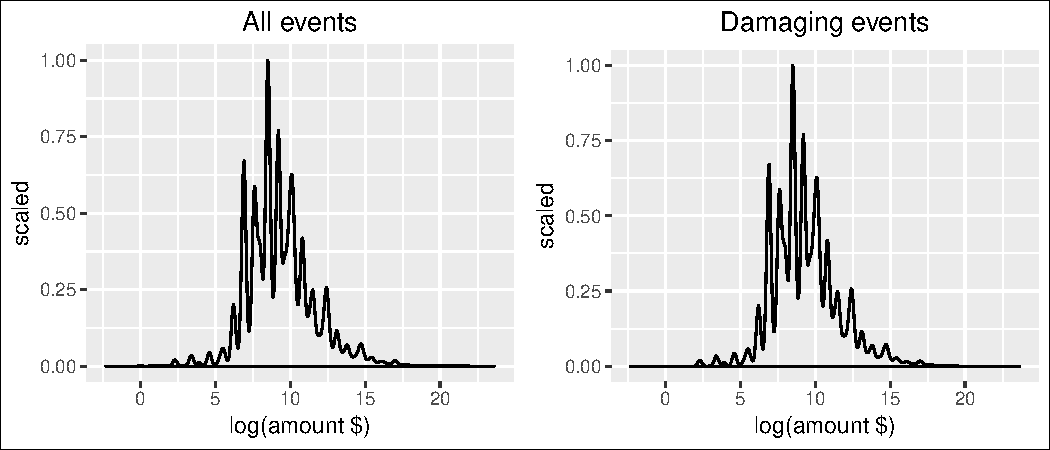
\includegraphics{readme_files/figure-latex/crop-distribution-1.pdf}
\caption{Population distribution for losses / occurrences}
\end{figure}

In this study, we looked on the 1\% most harmful occurrences.

\begin{longtable}[]{@{}rlllrlll@{}}
\caption{Worst property damaging occurrences, mean = \$1,137,697 and
median = \$10,000}\tabularnewline
\toprule
rank & event & magnitude & day & duration & state & countyname &
value\tabularnewline
\midrule
\endfirsthead
\toprule
rank & event & magnitude & day & duration & state & countyname &
value\tabularnewline
\midrule
\endhead
1 & TIDE & & 2005-08-29 & 0S & LOUISIANA & ORLEANS &
\$17,900,000,000\tabularnewline
2 & HURRICANE & & 2005-10-24 & 0S & FLORIDA & COASTAL.PALM.BEACH &
\$10,000,000,000\tabularnewline
3 & FLOOD & & 2012-10-29 & 0S & NEW JERSEY & EASTERN.OCEAN &
\$7,500,000,000\tabularnewline
4 & TIDE & & 2005-08-29 & 0S & MISSISSIPPI & HARRISON &
\$5,630,000,000\tabularnewline
5 & STORM & & 2001-06-05 & 0S & TEXAS & HARRIS &
\$5,030,000,000\tabularnewline
6 & FLOOD & & 2012-10-28 & 0S & NEW JERSEY & EASTERN.MONMOUTH &
\$5,000,000,000\tabularnewline
7 & FLOOD & & 2012-10-28 & 0S & NEW JERSEY & WESTERN.MONMOUTH &
\$5,000,000,000\tabularnewline
8 & HURRICANE & & 2004-09-13 & 0S & FLORIDA & COASTAL.ESCAMBIA &
\$4,000,000,000\tabularnewline
9 & TIDE & & 2008-09-12 & 0S & TEXAS & GALVESTON &
\$4,000,000,000\tabularnewline
10 & HURRICANE & & 2005-08-28 & 0S & LOUISIANA & ORLEANS &
\$3,560,000,000\tabularnewline
11 & TIDE & & 2005-08-29 & 0S & MISSISSIPPI & HANCOCK &
\$3,380,000,000\tabularnewline
12 & TIDE & & 2005-08-29 & 0S & LOUISIANA & ST..TAMMANY &
\$3,030,000,000\tabularnewline
13 & TIDE & & 2005-08-29 & 0S & LOUISIANA & LOWER.PLAQUEMINES &
\$3,030,000,000\tabularnewline
14 & TIDE & & 2005-08-29 & 0S & LOUISIANA & LOWER.ST..BERNARD &
\$3,020,000,000\tabularnewline
15 & TIDE & & 2005-08-29 & 0S & LOUISIANA & UPPER.ST..BERNARD &
\$3,020,000,000\tabularnewline
16 & FLOOD & & 1997-04-18 & 0S & NORTH DAKOTA & GRAND.FORKS &
\$3,000,000,000\tabularnewline
17 & HURRICANE & & 1999-09-15 & 0S & NORTH CAROLINA & ALAMANCE &
\$3,000,000,000\tabularnewline
18 & HURRICANE & & 2004-08-13 & 0S & FLORIDA & CHARLOTTE &
\$3,000,000,000\tabularnewline
19 & TIDE & & 2008-09-12 & 0S & TEXAS & HARRIS &
\$3,000,000,000\tabularnewline
20 & HURRICANE & & 2005-08-28 & 0S & MISSISSIPPI & HARRISON &
\$2,940,000,000\tabularnewline
\bottomrule
\end{longtable}

\begin{figure}[htbp]
\centering
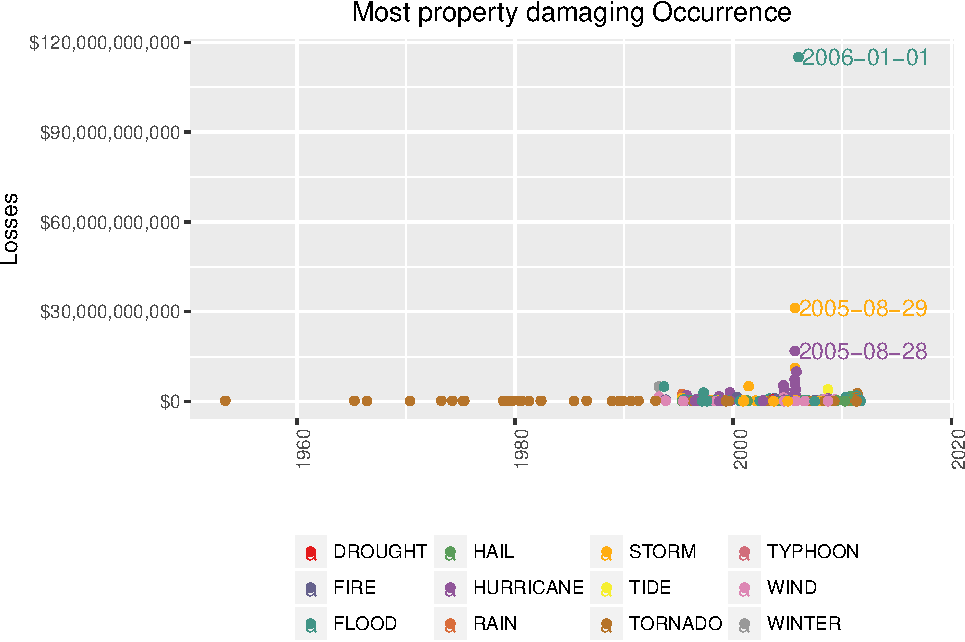
\includegraphics{readme_files/figure-latex/prop-single-plot-1.pdf}
\caption{Worst property damaging occurrences}
\end{figure}

The single most economic damaging event to properties was a
\textbf{TIDE, that occurred in LOUISIANA, ORLEANS, on 2005-08-29,
causing U\$ \$17,900,000,000 in losses}.

\subsubsection{Most Property Damaging event in all
time}\label{most-property-damaging-event-in-all-time}

Notice that are several occurrences of the same type of event along the
time.

Therefore, in order to know which is the worst type of event along all
the years, we summed up the losses caused by each one of occurrences of
this events.

Notice that we are interested only in the worst of them, ie, the ones
which are above the mean.

\begin{longtable}[]{@{}rllll@{}}
\caption{Total losses by event}\tabularnewline
\toprule
rank & event & total & mean & median\tabularnewline
\midrule
\endfirsthead
\toprule
rank & event & total & mean & median\tabularnewline
\midrule
\endhead
1 & HURRICANE & \$87,005,170,310 & \$11,737,195,233 &
\$229,971,300\tabularnewline
2 & FLOOD & \$82,920,597,380 & \$11,737,195,233 &
\$229,971,300\tabularnewline
3 & TORNADO & \$63,648,478,192 & \$11,737,195,233 &
\$229,971,300\tabularnewline
4 & TIDE & \$54,155,102,600 & \$11,737,195,233 &
\$229,971,300\tabularnewline
5 & HAIL & \$25,360,544,274 & \$11,737,195,233 &
\$229,971,300\tabularnewline
6 & WIND & \$24,868,014,778 & \$11,737,195,233 &
\$229,971,300\tabularnewline
7 & STORM & \$16,753,590,360 & \$11,737,195,233 &
\$229,971,300\tabularnewline
\bottomrule
\end{longtable}

\begin{figure}[htbp]
\centering
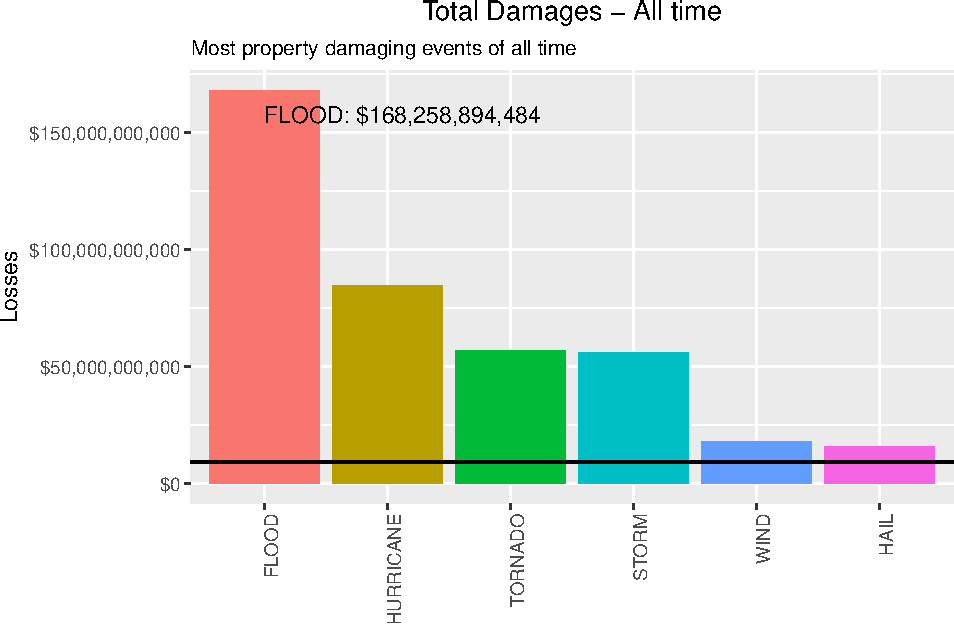
\includegraphics{readme_files/figure-latex/prop-all-plot-1.pdf}
\caption{Total Property Damages by event}
\end{figure}

The most property damaging event along the time is the
\textbf{HURRICANE. It has caused \$87,005,170,310 in losses.}

\subsubsection{Least property damaging
events}\label{least-property-damaging-events}

Just for curiosity, these are the less damaging events:

\begin{longtable}[]{@{}rll@{}}
\caption{Least property damaging events}\tabularnewline
\toprule
rank & event & total\tabularnewline
\midrule
\endfirsthead
\toprule
rank & event & total\tabularnewline
\midrule
\endhead
32 & OTHER & \$1,000\tabularnewline
31 & FUNNEL & \$123,100\tabularnewline
30 & DENSE SMOKE & \$130,000\tabularnewline
29 & RIP CURRENT & \$163,000\tabularnewline
28 & VOLCANIC ASH & \$500,000\tabularnewline
27 & DUST DEVIL & \$1,147,430\tabularnewline
26 & SEICHE & \$1,402,000\tabularnewline
25 & SLEET & \$3,084,000\tabularnewline
24 & AVALANCHE & \$4,058,050\tabularnewline
23 & WATERSPOUT & \$5,748,200\tabularnewline
\bottomrule
\end{longtable}

\subsection{Crop losses}\label{crop-losses}

\subsubsection{Most Crop Damaging event in a single
occurrence}\label{most-crop-damaging-event-in-a-single-occurrence}

In order to determine what were the most crop damaging events in a
single occurrence, we need to see how damages are distributed along the
occurrences.

On the other hand, damaging occurrences had to have damages above zero.

Now, among the damaging occurrences, we are interested in the ones whose
damages are above 99\% of the most common values.

Looking at this distribution, we can infer that \textbf{99.8\% of the
damaging occurrences caused up to \$197,450,000 in losses.}

\begin{figure}[htbp]
\centering
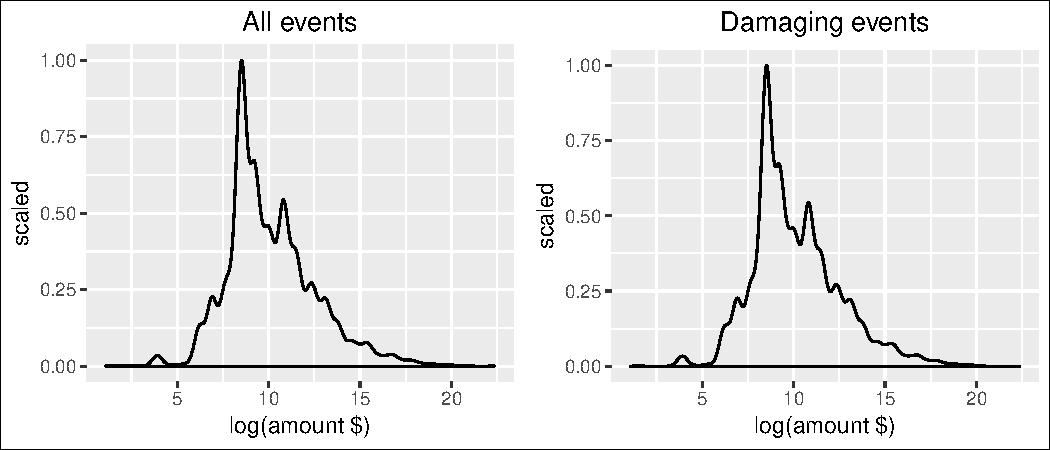
\includegraphics{readme_files/figure-latex/crop-distr-4-1.pdf}
\caption{Population distribution for losses / occurrences}
\end{figure}

In this study, we looked on the 1\% most harmful occurrences.

\begin{longtable}[]{@{}rlllrlll@{}}
\caption{Worst crops damaging occurrences, mean = \$1,783,319 and median
= \$20,000}\tabularnewline
\toprule
rank & event & magnitude & day & duration & state & countyname &
value\tabularnewline
\midrule
\endfirsthead
\toprule
rank & event & magnitude & day & duration & state & countyname &
value\tabularnewline
\midrule
\endhead
1 & DROUGHT & & 2014-12-01 & 0S & CALIFORNIA &
NORTHERN.SAN.JOAQUIN.VALLEY & \$1,500,000,000\tabularnewline
2 & DROUGHT & & 2011-06-01 & 0S & TEXAS & LUBBOCK &
\$1,050,000,000\tabularnewline
3 & DROUGHT & & 2006-01-01 & 0S & TEXAS & MONTAGUE &
\$1,000,000,000\tabularnewline
4 & DROUGHT & & 2007-06-01 & 0S & MISSISSIPPI & WARREN &
\$700,000,000\tabularnewline
5 & COLD & & 2007-01-11 & 0S & CALIFORNIA & SE.S.J..VALLEY &
\$568,600,000\tabularnewline
6 & DROUGHT & & 2000-11-01 & 0S & TEXAS & PARMER &
\$515,000,000\tabularnewline
7 & DROUGHT & & 1998-07-06 & 0S & OKLAHOMA & CHOCTAW &
\$500,000,000\tabularnewline
8 & DROUGHT & & 1999-07-01 & 0S & PENNSYLVANIA & POTTER &
\$500,000,000\tabularnewline
9 & HURRICANE & & 1999-09-15 & 0S & NORTH CAROLINA & ALAMANCE &
\$500,000,000\tabularnewline
10 & FLOOD & & 2000-10-03 & 0S & FLORIDA & COASTAL.DADE &
\$500,000,000\tabularnewline
11 & FLOOD & & 2007-07-01 & 0S & MISSOURI & HENRY &
\$500,000,000\tabularnewline
12 & WIND & & 1998-12-20 & 0S & CALIFORNIA & SOUTHERN.SAN.JOAQUIN.VALLEY
& \$490,500,000\tabularnewline
13 & DROUGHT & & 1998-12-01 & 0S & TEXAS & YOAKUM &
\$450,000,000\tabularnewline
14 & HURRICANE & & 2005-08-25 & 0S & FLORIDA & COASTAL.DADE &
\$423,000,000\tabularnewline
15 & DROUGHT & & 2001-12-01 & 0S & TEXAS & PARMER &
\$420,000,000\tabularnewline
16 & DROUGHT & & 2007-09-01 & 0S & GEORGIA & BALDWIN &
\$344,000,000\tabularnewline
17 & DROUGHT & & 2006-02-01 & 0S & TEXAS & FANNIN &
\$300,000,000\tabularnewline
18 & COLD & & 2010-01-10 & 0S & FLORIDA & INLAND.COLLIER.COUNTY &
\$300,000,000\tabularnewline
19 & COLD & & 2010-01-10 & 0S & FLORIDA & INLAND.MIAMI.DADE &
\$286,000,000\tabularnewline
20 & DROUGHT & & 1998-12-01 & 0S & TEXAS & ANDREWS &
\$250,000,000\tabularnewline
\bottomrule
\end{longtable}

\begin{figure}[htbp]
\centering
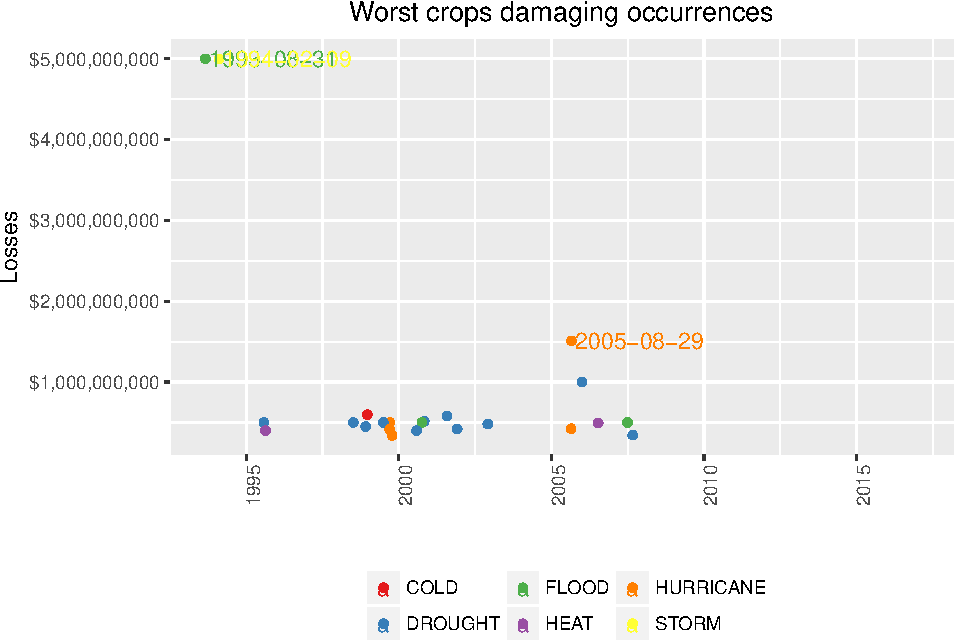
\includegraphics{readme_files/figure-latex/crop-single-plot-1.pdf}
\caption{Worst crops damaging occurrences}
\end{figure}

The single most economic damaging event to crops was a \textbf{DROUGHT,
that occurred in CALIFORNIA, NORTHERN.SAN.JOAQUIN.VALLEY, on 2014-12-01,
causing U\$ \$1,500,000,000 in losses.}

\subsubsection{Most Crop Damaging event in all
time}\label{most-crop-damaging-event-in-all-time}

Notice that are several occurrences of the same type of event along the
time.

Therefore, in order to know which is the worst type of event along all
the years, we summed up the losses caused by each one of occurrences of
this events.

Notice that we are interested only in the worst of them, ie, the ones
which are above the mean.

\begin{longtable}[]{@{}rllll@{}}
\caption{Total losses by event}\tabularnewline
\toprule
rank & event & total & mean & median\tabularnewline
\midrule
\endfirsthead
\toprule
rank & event & total & mean & median\tabularnewline
\midrule
\endhead
1 & DROUGHT & \$27,454,862,620 & \$2,957,587,920 &
\$450,448,110\tabularnewline
2 & FLOOD & \$7,750,252,370 & \$2,957,587,920 &
\$450,448,110\tabularnewline
3 & HURRICANE & \$5,341,874,800 & \$2,957,587,920 &
\$450,448,110\tabularnewline
4 & COLD & \$4,919,893,200 & \$2,957,587,920 &
\$450,448,110\tabularnewline
5 & WIND & \$3,679,520,230 & \$2,957,587,920 &
\$450,448,110\tabularnewline
6 & HAIL & \$3,657,650,043 & \$2,957,587,920 &
\$450,448,110\tabularnewline
\bottomrule
\end{longtable}

\begin{figure}[htbp]
\centering
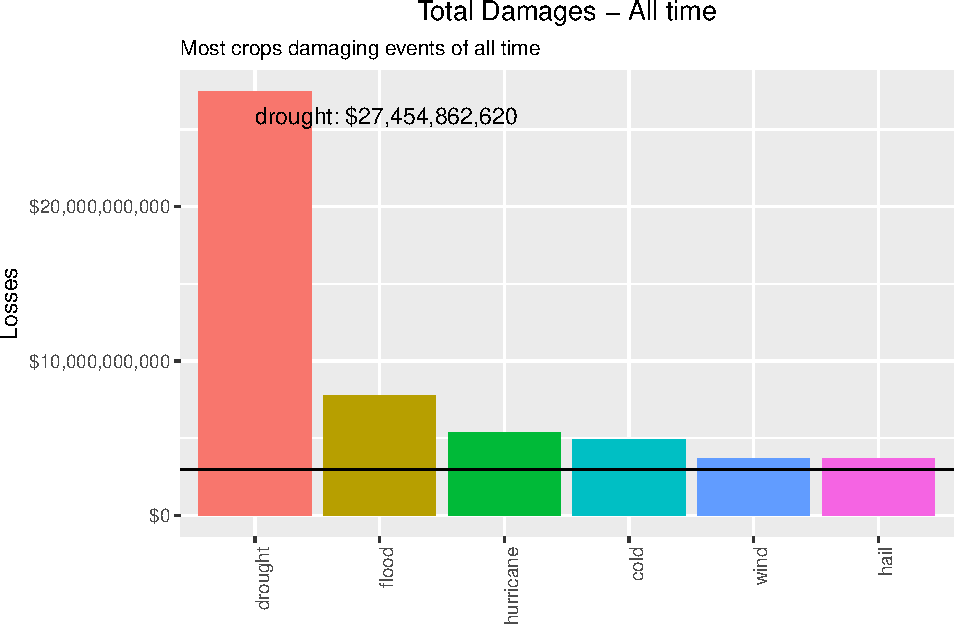
\includegraphics{readme_files/figure-latex/crop-all-plot-1.pdf}
\caption{Total Crop Damages by event}
\end{figure}

The most crop damaging event along the time is the \textbf{DROUGHT. It
has caused \$27,454,862,620 in losses.}

\subsubsection{Least crops damaging
events}\label{least-crops-damaging-events}

Just for curiosity, lets show now what are the less damaging among the
events:

\begin{longtable}[]{@{}rll@{}}
\caption{Least crops damaging events}\tabularnewline
\toprule
rank & event & total\tabularnewline
\midrule
\endfirsthead
\toprule
rank & event & total\tabularnewline
\midrule
\endhead
19 & SLIDE & \$17,000\tabularnewline
18 & TSUNAMI & \$20,000\tabularnewline
17 & TIDE & \$955,000\tabularnewline
16 & BLIZZARD & \$7,060,000\tabularnewline
15 & LIGHTNING & \$7,422,640\tabularnewline
14 & DEBRIS FLOW & \$20,001,500\tabularnewline
13 & WINTER & \$46,924,000\tabularnewline
12 & SNOW & \$91,145,900\tabularnewline
11 & FIRE & \$447,668,860\tabularnewline
10 & TORNADO & \$450,448,110\tabularnewline
\bottomrule
\end{longtable}

\section{Most aflicted locations}\label{most-aflicted-locations}

We have determined what locations had the worst outcome from those
events, both in terms of human health and economic losses.

Unfortunatelly, these has been the worst counties for living in:

\subsection{Worst fatality count}\label{worst-fatality-count}

\begin{longtable}[]{@{}rllrrll@{}}
\caption{Total fatalities by county}\tabularnewline
\toprule
rank & state & countyname & fatalities & injuries & prop.dmg &
crop.dmg\tabularnewline
\midrule
\endfirsthead
\toprule
rank & state & countyname & fatalities & injuries & prop.dmg &
crop.dmg\tabularnewline
\midrule
\endhead
1 & LOUISIANA & ORLEANS & 649 & 99 & \$21,614,049,550 &
\$0\tabularnewline
2 & ILLINOIS & COOK & 565 & 912 & \$670,237,350 & \$0\tabularnewline
3 & PENNSYLVANIA & PHILADELPHIA & 387 & 455 & \$52,680,980 &
\$0\tabularnewline
4 & NEVADA & LAS.VEGAS.VALLEY & 263 & 601 & \$13,162,000 &
\$0\tabularnewline
5 & TEXAS & HARRIS & 216 & 2825 & \$10,890,439,870 &
\$7,442,000\tabularnewline
6 & MISSOURI & JASPER & 178 & 1273 & \$2,864,021,330 &
\$46,475,500\tabularnewline
7 & TEXAS & DALLAS & 149 & 1757 & \$1,946,192,730 &
\$1,405,000\tabularnewline
8 & LOUISIANA & LOWER.ST..BERNARD & 140 & 0 & \$4,845,022,000 &
\$0\tabularnewline
9 & TEXAS & MCLENNAN & 127 & 657 & \$65,138,600 &
\$1,710,500\tabularnewline
10 & MICHIGAN & GENESEE & 123 & 962 & \$107,151,750 &
\$6,300,000\tabularnewline
\bottomrule
\end{longtable}

The county with the biggest fatality count is \textbf{ORLEANS, in
LOUISIANA, with 649 people killed.}

\subsection{Worst injuries count}\label{worst-injuries-count}

\begin{longtable}[]{@{}rllrrll@{}}
\caption{Total injuries by county}\tabularnewline
\toprule
rank & state & countyname & fatalities & injuries & prop.dmg &
crop.dmg\tabularnewline
\midrule
\endfirsthead
\toprule
rank & state & countyname & fatalities & injuries & prop.dmg &
crop.dmg\tabularnewline
\midrule
\endhead
1 & MISSOURI & ST..LOUIS & 65 & 3144 & \$1,461,882,880 &
\$10,500\tabularnewline
2 & TEXAS & HARRIS & 216 & 2825 & \$10,890,439,870 &
\$7,442,000\tabularnewline
3 & MISSOURI & ST..LOUIS. & 118 & 2701 & \$79,552,000 &
\$5,000\tabularnewline
4 & TEXAS & WICHITA & 55 & 1853 & \$310,822,880 & \$0\tabularnewline
5 & TEXAS & DALLAS & 149 & 1757 & \$1,946,192,730 &
\$1,405,000\tabularnewline
6 & ALABAMA & JEFFERSON & 117 & 1699 & \$2,037,082,100 &
\$3,355,000\tabularnewline
7 & MASSACHUSETTS & WORCESTER & 96 & 1292 & \$286,072,530 &
\$0\tabularnewline
8 & OHIO & GREENE & 40 & 1278 & \$289,967,757 & \$540,000\tabularnewline
9 & MISSOURI & JASPER & 178 & 1273 & \$2,864,021,330 &
\$46,475,500\tabularnewline
10 & OKLAHOMA & OKLAHOMA & 79 & 1253 & \$1,356,088,290 &
\$8,330,000\tabularnewline
\bottomrule
\end{longtable}

The county with the biggest injuries count is \textbf{ST..LOUIS, in
MISSOURI, with 3144 people injuried.}

\subsection{Worst property losses}\label{worst-property-losses}

\begin{longtable}[]{@{}rllrrll@{}}
\caption{Total property losses by county}\tabularnewline
\toprule
rank & state & countyname & fatalities & injuries & prop.dmg &
crop.dmg\tabularnewline
\midrule
\endfirsthead
\toprule
rank & state & countyname & fatalities & injuries & prop.dmg &
crop.dmg\tabularnewline
\midrule
\endhead
1 & LOUISIANA & ORLEANS & 649 & 99 & \$21,614,049,550 &
\$0\tabularnewline
2 & TEXAS & HARRIS & 216 & 2825 & \$10,890,439,870 &
\$7,442,000\tabularnewline
3 & FLORIDA & COASTAL.PALM.BEACH & 5 & 7 & \$10,828,630,000 &
\$75,000,000\tabularnewline
4 & MISSISSIPPI & HARRISON & 110 & 90 & \$8,870,659,460 &
\$0\tabularnewline
5 & NEW JERSEY & EASTERN.OCEAN & 16 & 112 & \$8,116,441,690 &
\$10\tabularnewline
6 & NEW JERSEY & EASTERN.MONMOUTH & 13 & 397 & \$6,527,278,550 &
\$0\tabularnewline
7 & LOUISIANA & ST..TAMMANY & 8 & 89 & \$5,677,622,950 &
\$0\tabularnewline
8 & FLORIDA & COASTAL.ESCAMBIA & 14 & 0 & \$5,632,695,000 &
\$25,300,000\tabularnewline
9 & TEXAS & GALVESTON & 43 & 259 & \$5,358,909,770 &
\$109,602,000\tabularnewline
10 & NEW JERSEY & WESTERN.MONMOUTH & 6 & 84 & \$5,267,488,450 &
\$0\tabularnewline
\bottomrule
\end{longtable}

The county with the biggest property losses is \textbf{ORLEANS, in
LOUISIANA, with \$21,614,049,550 in losses.}

\subsection{Worst crops losses}\label{worst-crops-losses}

\begin{longtable}[]{@{}rllrrll@{}}
\caption{Total crops losses by county}\tabularnewline
\toprule
rank & state & countyname & fatalities & injuries & prop.dmg &
crop.dmg\tabularnewline
\midrule
\endfirsthead
\toprule
rank & state & countyname & fatalities & injuries & prop.dmg &
crop.dmg\tabularnewline
\midrule
\endhead
1 & TEXAS & LUBBOCK & 37 & 679 & \$2,007,426,360 &
\$2,439,945,000\tabularnewline
2 & TEXAS & MONTAGUE & 5 & 42 & \$118,971,700 &
\$1,963,106,500\tabularnewline
3 & CALIFORNIA & NORTHERN.SAN.JOAQUIN.VALLEY & 14 & 25 & \$5,948,500 &
\$1,520,000,000\tabularnewline
4 & TEXAS & PARMER & 1 & 23 & \$44,654,090 &
\$1,181,360,000\tabularnewline
5 & FLORIDA & COASTAL.DADE & 10 & 1 & \$693,020,000 &
\$1,168,000,000\tabularnewline
6 & CALIFORNIA & SE.S.J..VALLEY & 25 & 64 & \$5,742,300 &
\$992,123,000\tabularnewline
7 & MISSISSIPPI & WARREN & 43 & 341 & \$312,674,880 &
\$728,657,000\tabularnewline
8 & CALIFORNIA & E.CENTRAL.S.J..VALLEY & 43 & 73 & \$6,936,800 &
\$547,162,000\tabularnewline
9 & CALIFORNIA & SOUTHERN.SAN.JOAQUIN.VALLEY & 1 & 22 & \$18,657,000 &
\$517,800,000\tabularnewline
10 & NORTH CAROLINA & ALAMANCE & 2 & 8 & \$3,005,157,200 &
\$503,166,000\tabularnewline
\bottomrule
\end{longtable}

The county with the biggest croperty losses is \textbf{LUBBOCK, in
TEXAS, with \$2,439,945,000 in losses.}

\section{Results}\label{results}

\subsection{Population Health}\label{population-health}

\begin{figure}[htbp]
\centering
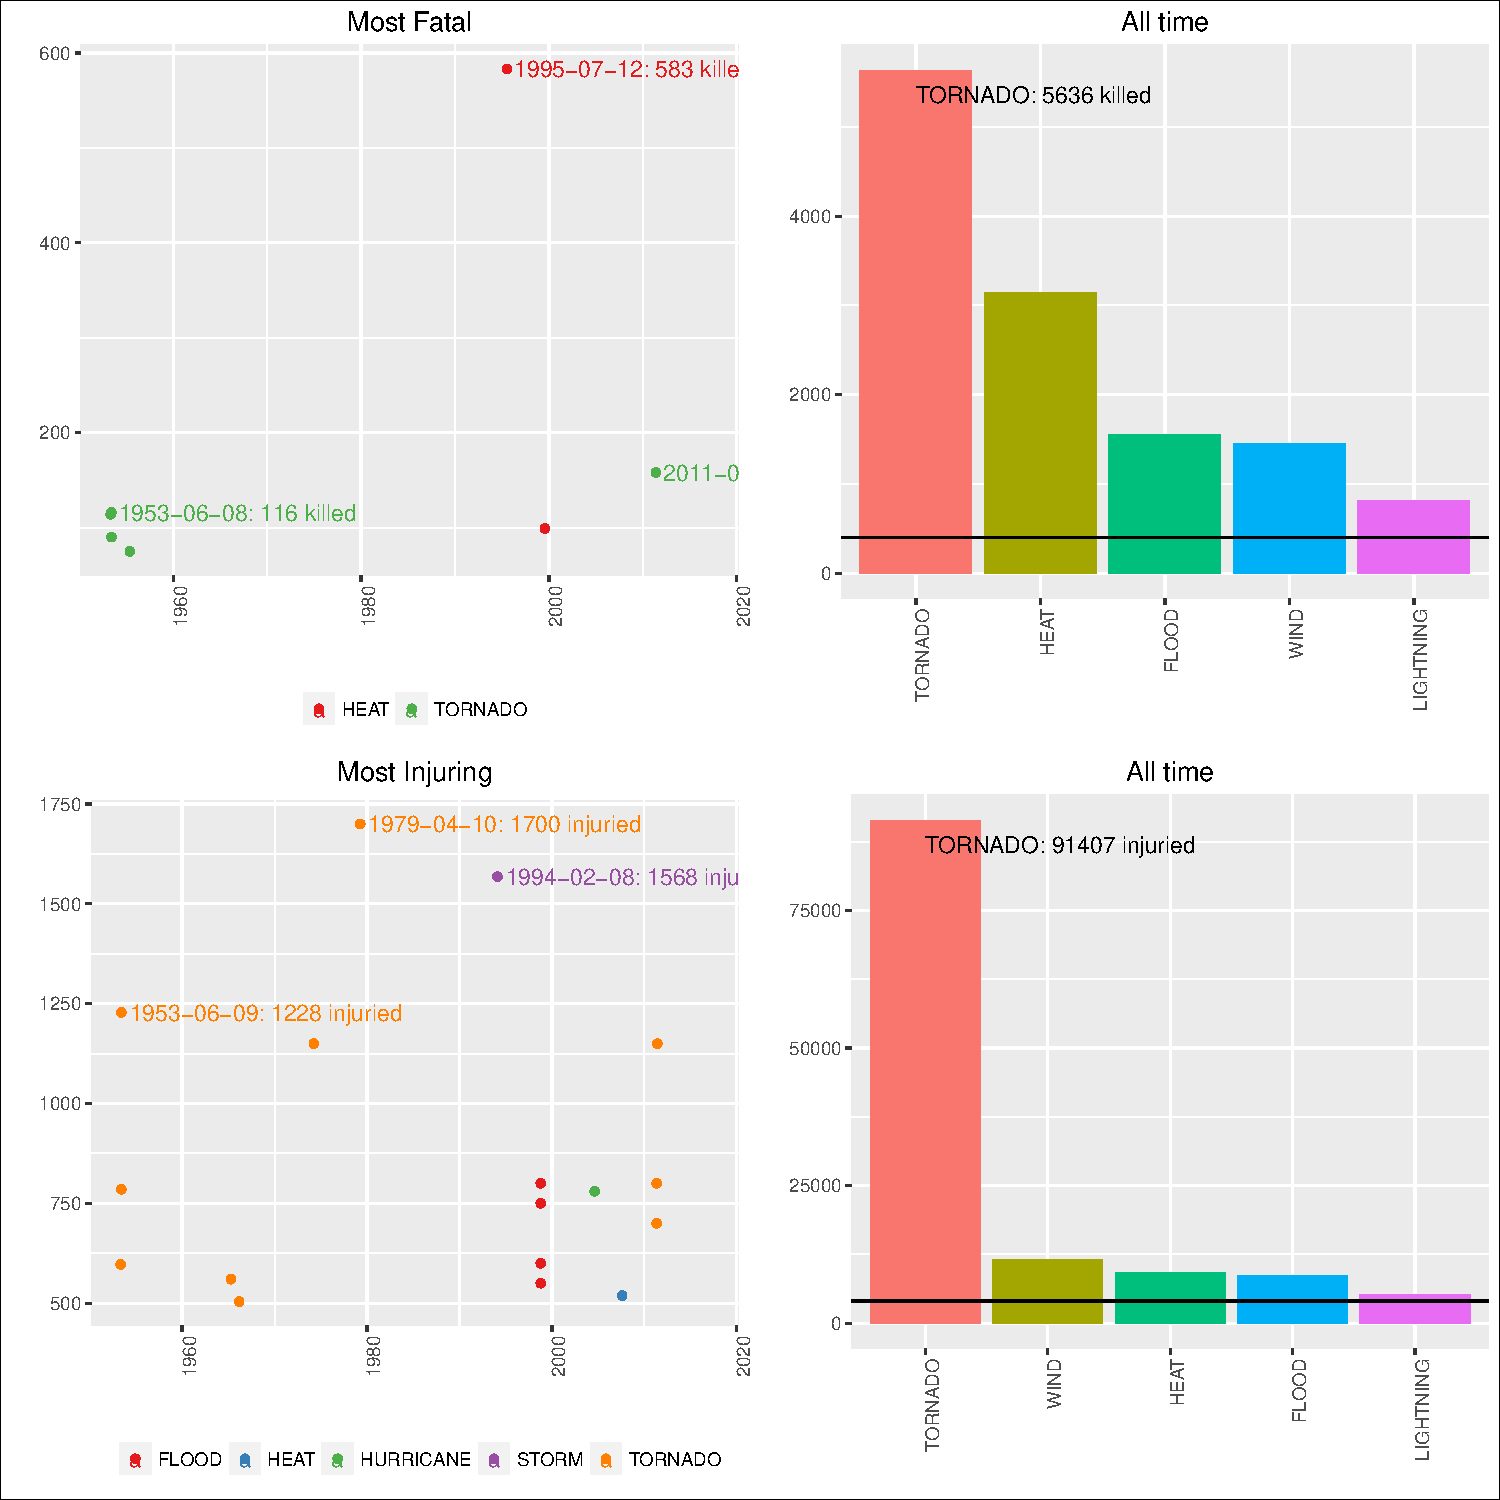
\includegraphics{readme_files/figure-latex/health-plot-1.pdf}
\caption{Population Health: fatalities and injuries}
\end{figure}

The single most fatal event was a \textbf{HURRICANE, that occurred in
LOUISIANA, ORLEANS, on 2005-08-28, killing 638 people.}

The most fatal event along the time is the \textbf{TORNADO. It has
killed 5873 people until now.}

The single most injuring event was a \textbf{HURRICANE, that occurred in
TEXAS, HARRIS, on 2008-09-12, injuring 2400 people.}

The most injuring event along the time is the \textbf{TORNADO. It has
injuried 94614 people until now.}

\subsection{Economic Damages}\label{economic-damages}

\begin{figure}[htbp]
\centering
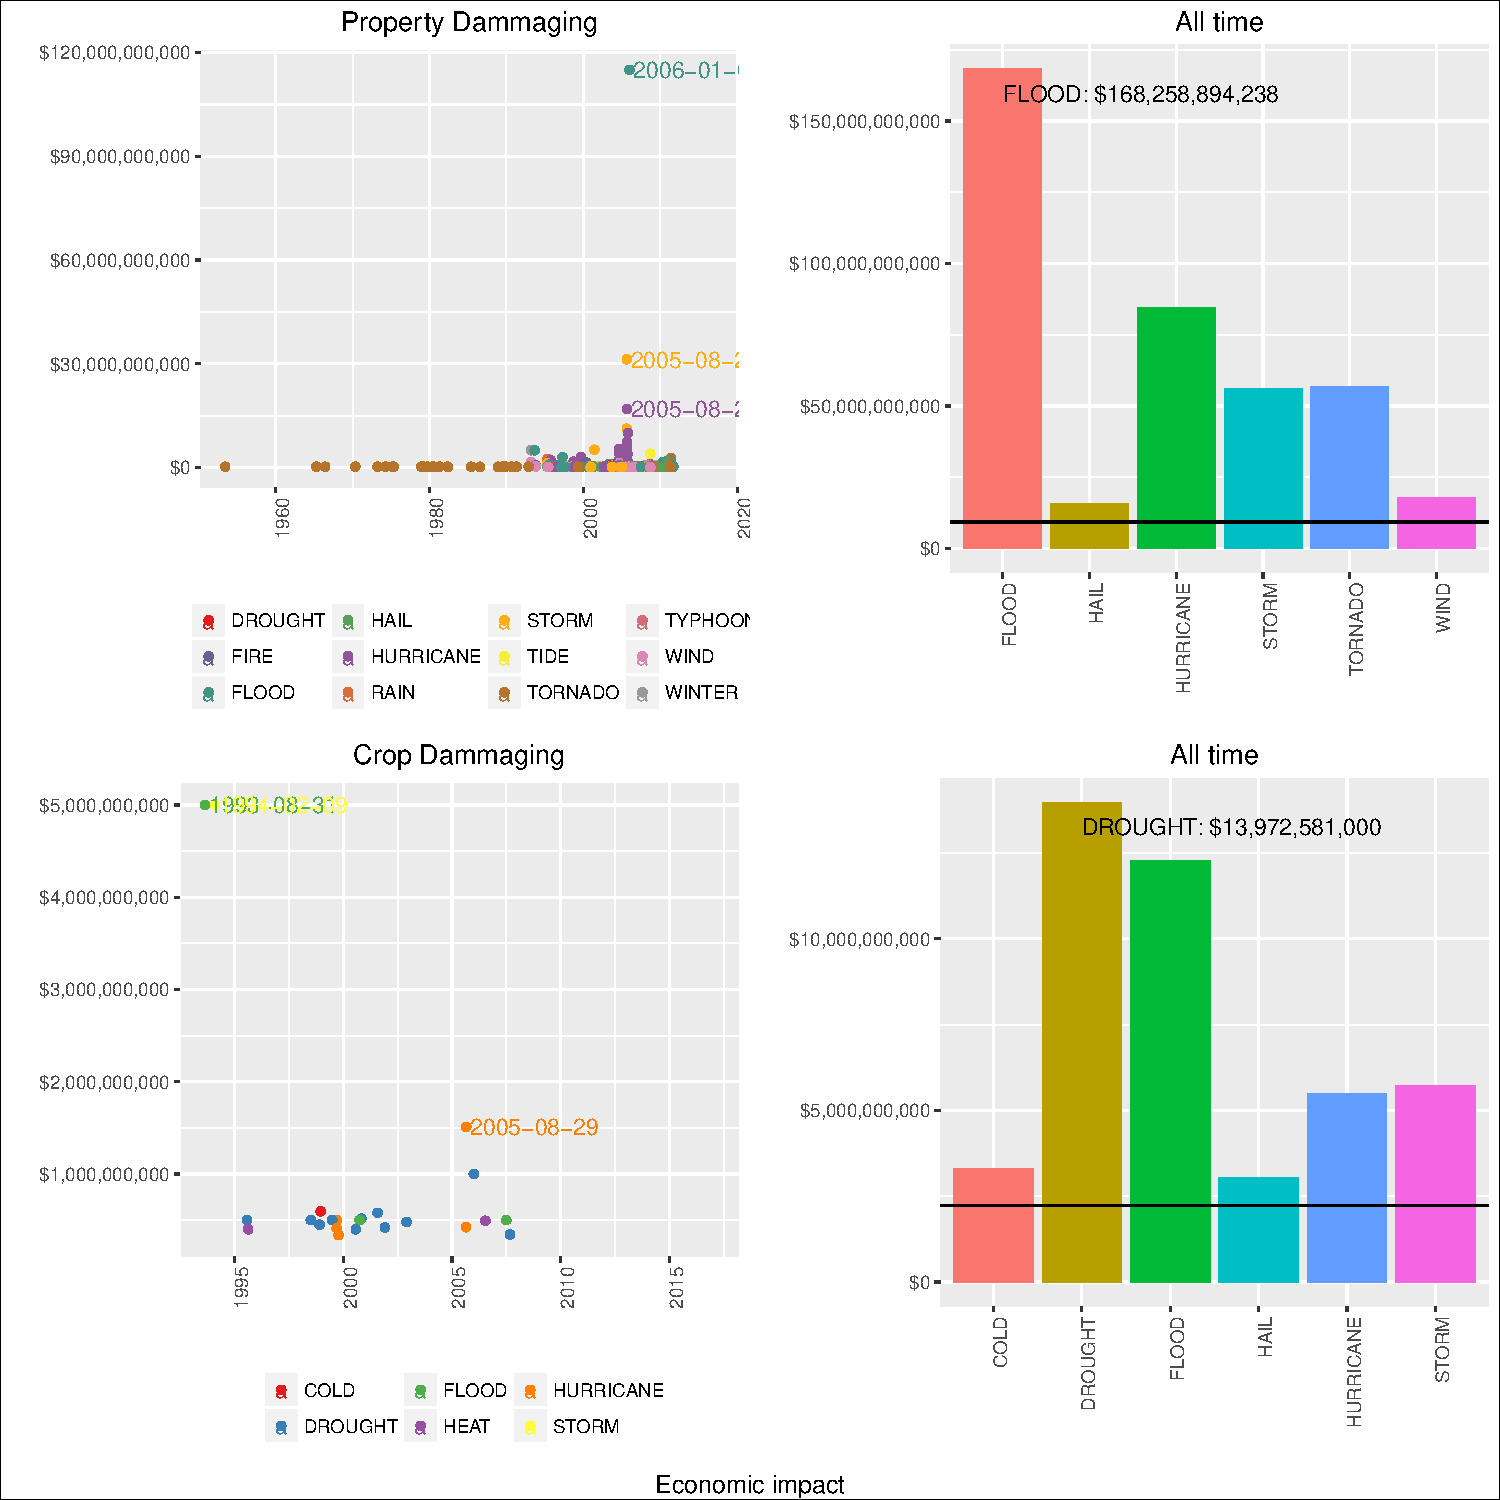
\includegraphics{readme_files/figure-latex/economic-plot-1.pdf}
\caption{Economic Damages: property and crops}
\end{figure}

The single most economic damaging event to properties was a
\textbf{TIDE, that occurred in LOUISIANA, ORLEANS, on 2005-08-29,
causing U\$ \$17,900,000,000 in losses}.

The most property damaging event along the time is the
\textbf{HURRICANE. It has caused \$87,005,170,310 in losses.}

The single most economic damaging event to crops was a \textbf{DROUGHT,
that occurred in CALIFORNIA, NORTHERN.SAN.JOAQUIN.VALLEY, on 2014-12-01,
causing U\$ \$1,500,000,000 in losses}.

The most crop damaging event along the time is the \textbf{DROUGHT. It
has caused \$27,454,862,620 in losses.}

\subsection{Most aflicted locations}\label{most-aflicted-locations-1}

The county with the biggest fatality count is \textbf{ORLEANS, in
LOUISIANA, with 649 people killed.}

The county with the biggest injuries count is \textbf{ST..LOUIS, in
MISSOURI, with 3144 people injuried.}

The county with the biggest property losses is \textbf{ORLEANS, in
LOUISIANA, with \$21,614,049,550 in losses.}

The county with the biggest croperty losses is \textbf{LUBBOCK, in
TEXAS, with \$2,439,945,000 in losses.}

\subsection{Distribution of data}\label{distribution-of-data}

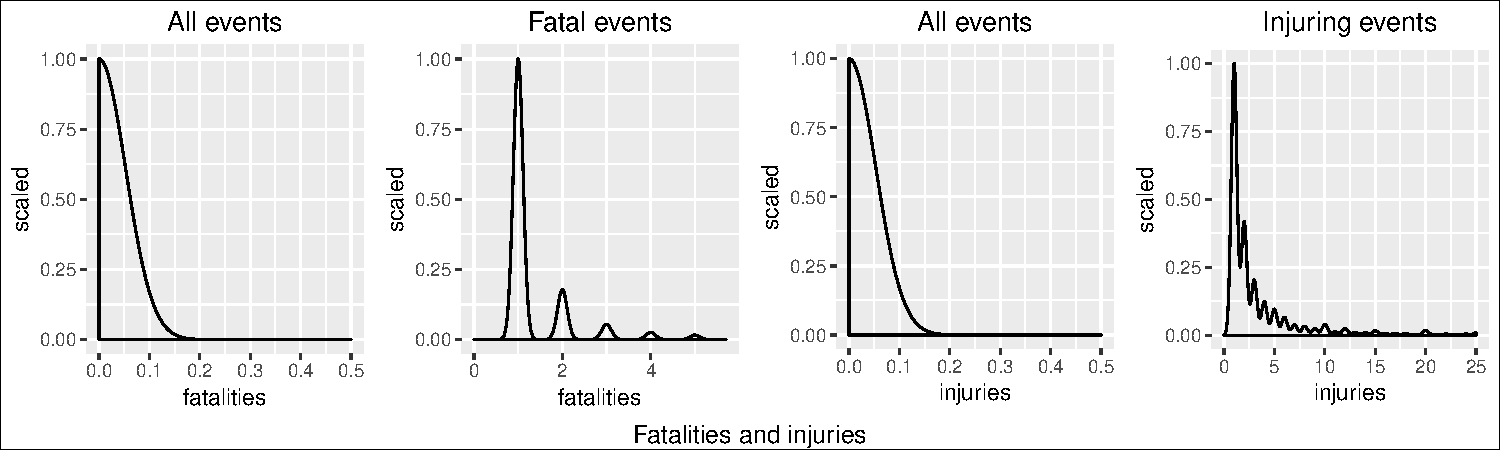
\includegraphics{readme_files/figure-latex/distribution-1.pdf}
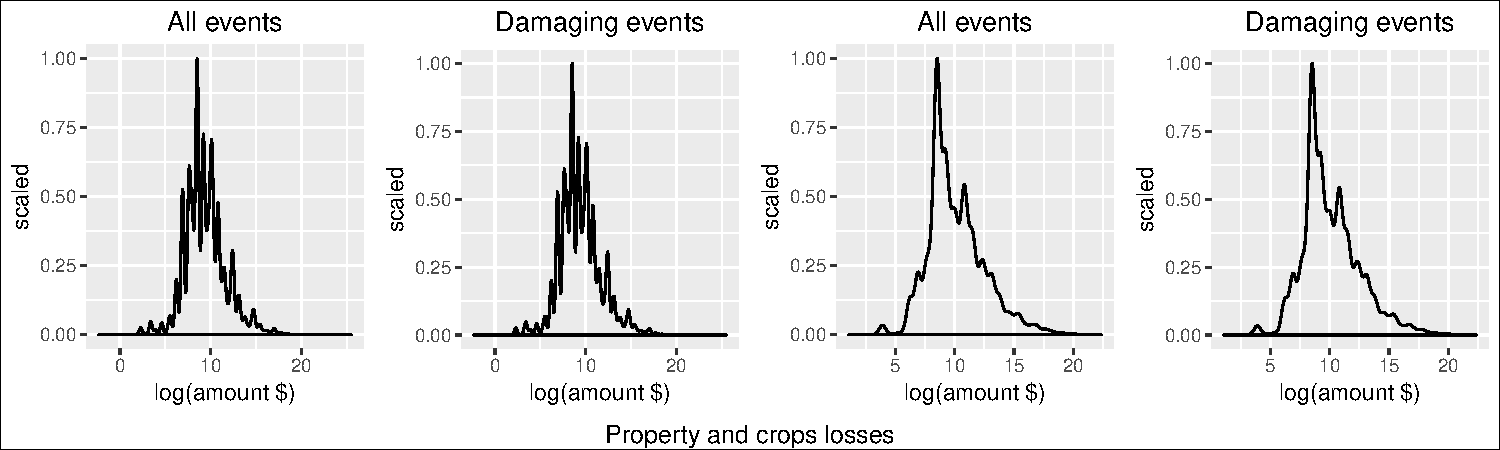
\includegraphics{readme_files/figure-latex/distribution-2.pdf}


\end{document}
